\documentclass[11pt,addpoints,answers]{exam}
%DIF LATEXDIFF DIFFERENCE FILE
%DIF DEL latex_template/hw7.tex   Fri Apr  3 05:01:36 2020
%DIF ADD new.tex                  Mon Apr  6 00:08:00 2020
%\documentclass[11pt]{article}
\usepackage[margin=1in]{geometry}
\usepackage{amsmath, amsfonts}
\usepackage{enumerate}
\usepackage{graphicx}
\usepackage{titling}
\usepackage{url}
\usepackage{xfrac}
% \usepackage{fancyhdr} % CONFLICTS with the exam class
\usepackage{geometry}
\usepackage{graphicx}
\usepackage{natbib}
\usepackage{amsmath}
\usepackage{amssymb}
\usepackage{amsthm}
\usepackage{paralist}
\usepackage{epstopdf}
\usepackage{tabularx}
\usepackage{longtable}
\usepackage{multirow}
\usepackage{multicol}
\usepackage[colorlinks=true,urlcolor=blue]{hyperref}
\usepackage{fancyvrb}
%DIF 25d25
%DIF < \usepackage{algorithm}
%DIF -------
\usepackage{algorithmic}
\usepackage{float}
\usepackage{paralist}
%\usepackage{xcolor}
\usepackage{enumerate}
\usepackage{array}
\usepackage{times}
\usepackage{url}
\usepackage{comment}
\usepackage{environ}
\usepackage{times}
\usepackage{textcomp}
\usepackage{caption}
\usepackage[colorlinks=true,urlcolor=blue]{hyperref}
\usepackage{listings}
\usepackage{parskip} % For NIPS style paragraphs.
\usepackage[compact]{titlesec} % Less whitespace around titles
\usepackage[inline]{enumitem} % For inline enumerate* and itemize*
\usepackage{datetime}
\usepackage{comment}
% \usepackage{minted}
\usepackage{lastpage}
\usepackage{color}
\usepackage[dvipsnames]{xcolor}
\usepackage[ruled]{algorithm2e}
%DIF 51d50
%DIF < \usepackage{listings}
%DIF -------
\usepackage{tikz}
\usetikzlibrary{shapes,decorations,bayesnet}
%\usepackage{framed}
\usepackage{booktabs}
\usepackage{cprotect}
%\usepackage{xcolor}
\usepackage{verbatimbox}
\usepackage[many]{tcolorbox}
\usepackage{cancel}
\usepackage{wasysym}
\usepackage{mdframed}
\usepackage{subcaption}
\usepackage{bm}
\usetikzlibrary{arrows,automata}
\usetikzlibrary{shapes.geometric}

%%%%%%%%%%%%%%%%%%%%%%%%%%%%%%%%%%%%%%%%%%%
% Formatting for \CorrectChoice of "exam" %
%%%%%%%%%%%%%%%%%%%%%%%%%%%%%%%%%%%%%%%%%%%

\CorrectChoiceEmphasis{}
\checkedchar{\blackcircle}

%%%%%%%%%%%%%%%%%%%%%%%%%%%%%%%%%%%%%%%%%%%
% Better numbering                        %
%%%%%%%%%%%%%%%%%%%%%%%%%%%%%%%%%%%%%%%%%%%

\numberwithin{equation}{section} % Number equations within sections (i.e. 1.1, 1.2, 2.1, 2.2 instead of 1, 2, 3, 4)
\numberwithin{figure}{section} % Number figures within sections (i.e. 1.1, 1.2, 2.1, 2.2 instead of 1, 2, 3, 4)
\numberwithin{table}{section} % Number tables within sections (i.e. 1.1, 1.2, 2.1, 2.2 instead of 1, 2, 3, 4)


%%%%%%%%%%%%%%%%%%%%%%%%%%%%%%%%%%%%%%%%%%%
% Common Math Commands                    %
%%%%%%%%%%%%%%%%%%%%%%%%%%%%%%%%%%%%%%%%%%%

%%%%%%%%%%%%%%%%%%%%%%%%%%%%%%%%%%%%%%%%%%
% Custom commands                        %
%%%%%%%%%%%%%%%%%%%%%%%%%%%%%%%%%%%%%%%%%%

\newcommand{\vc}[1]{\boldsymbol{#1}}
\newcommand{\adj}[1]{\frac{d J}{d #1}}
%DIF 94c92
%DIF < \newcommand{\chain}[2]{\adj{#3} = \adj{#1}\frac{d #1}{d #2}}
%DIF -------
\newcommand{\chain}[2]{\adj{##3} = \adj{##1}\frac{d ##1}{d ##2}} %DIF > 
%DIF -------

% mathcal
\newcommand{\Ac}{\mathcal{A}}
\newcommand{\Bc}{\mathcal{B}}
\newcommand{\Cc}{\mathcal{C}}
\newcommand{\Dc}{\mathcal{D}}
\newcommand{\Ec}{\mathcal{E}}
\newcommand{\Fc}{\mathcal{F}}
\newcommand{\Gc}{\mathcal{G}}
\newcommand{\Hc}{\mathcal{H}}
\newcommand{\Ic}{\mathcal{I}}
\newcommand{\Jc}{\mathcal{J}}
\newcommand{\Kc}{\mathcal{K}}
\newcommand{\Lc}{\mathcal{L}}
\newcommand{\Mc}{\mathcal{M}}
\newcommand{\Nc}{\mathcal{N}}
\newcommand{\Oc}{\mathcal{O}}
\newcommand{\Pc}{\mathcal{P}}
\newcommand{\Qc}{\mathcal{Q}}
\newcommand{\Rc}{\mathcal{R}}
\newcommand{\Sc}{\mathcal{S}}
\newcommand{\Tc}{\mathcal{T}}
\newcommand{\Uc}{\mathcal{U}}
\newcommand{\Vc}{\mathcal{V}}
\newcommand{\Wc}{\mathcal{W}}
\newcommand{\Xc}{\mathcal{X}}
\newcommand{\Yc}{\mathcal{Y}}
\newcommand{\Zc}{\mathcal{Z}}

% mathbb
\newcommand{\Ab}{\mathbb{A}}
\newcommand{\Bb}{\mathbb{B}}
\newcommand{\Cb}{\mathbb{C}}
\newcommand{\Db}{\mathbb{D}}
\newcommand{\Eb}{\mathbb{E}}
\newcommand{\Fb}{\mathbb{F}}
\newcommand{\Gb}{\mathbb{G}}
\newcommand{\Hb}{\mathbb{H}}
\newcommand{\Ib}{\mathbb{I}}
\newcommand{\Jb}{\mathbb{J}}
\newcommand{\Kb}{\mathbb{K}}
\newcommand{\Lb}{\mathbb{L}}
\newcommand{\Mb}{\mathbb{M}}
\newcommand{\Nb}{\mathbb{N}}
\newcommand{\Ob}{\mathbb{O}}
\newcommand{\Pb}{\mathbb{P}}
\newcommand{\Qb}{\mathbb{Q}}
\newcommand{\Rb}{\mathbb{R}}
\newcommand{\Sb}{\mathbb{S}}
\newcommand{\Tb}{\mathbb{T}}
\newcommand{\Ub}{\mathbb{U}}
\newcommand{\Vb}{\mathbb{V}}
\newcommand{\Wb}{\mathbb{W}}
\newcommand{\Xb}{\mathbb{X}}
\newcommand{\Yb}{\mathbb{Y}}
\newcommand{\Zb}{\mathbb{Z}}

% mathbf lowercase
\newcommand{\av}{\mathbf{a}}
\newcommand{\bv}{\mathbf{b}}
\newcommand{\cv}{\mathbf{c}}
\newcommand{\dv}{\mathbf{d}}
\newcommand{\ev}{\mathbf{e}}
\newcommand{\fv}{\mathbf{f}}
\newcommand{\gv}{\mathbf{g}}
\newcommand{\hv}{\mathbf{h}}
\newcommand{\iv}{\mathbf{i}}
\newcommand{\jv}{\mathbf{j}}
\newcommand{\kv}{\mathbf{k}}
\newcommand{\lv}{\mathbf{l}}
\newcommand{\mv}{\mathbf{m}}
\newcommand{\nv}{\mathbf{n}}
\newcommand{\ov}{\mathbf{o}}
\newcommand{\pv}{\mathbf{p}}
\newcommand{\qv}{\mathbf{q}}
\newcommand{\rv}{\mathbf{r}}
\newcommand{\sv}{\mathbf{s}}
\newcommand{\tv}{\mathbf{t}}
\newcommand{\uv}{\mathbf{u}}
\newcommand{\vv}{\mathbf{v}}
\newcommand{\wv}{\mathbf{w}}
\newcommand{\xv}{\mathbf{x}}
\newcommand{\yv}{\mathbf{y}}
\newcommand{\zv}{\mathbf{z}}

% mathbf uppercase
\newcommand{\Av}{\mathbf{A}}
\newcommand{\Bv}{\mathbf{B}}
\newcommand{\Cv}{\mathbf{C}}
\newcommand{\Dv}{\mathbf{D}}
\newcommand{\Ev}{\mathbf{E}}
\newcommand{\Fv}{\mathbf{F}}
\newcommand{\Gv}{\mathbf{G}}
\newcommand{\Hv}{\mathbf{H}}
\newcommand{\Iv}{\mathbf{I}}
\newcommand{\Jv}{\mathbf{J}}
\newcommand{\Kv}{\mathbf{K}}
\newcommand{\Lv}{\mathbf{L}}
\newcommand{\Mv}{\mathbf{M}}
\newcommand{\Nv}{\mathbf{N}}
\newcommand{\Ov}{\mathbf{O}}
\newcommand{\Pv}{\mathbf{P}}
\newcommand{\Qv}{\mathbf{Q}}
\newcommand{\Rv}{\mathbf{R}}
\newcommand{\Sv}{\mathbf{S}}
\newcommand{\Tv}{\mathbf{T}}
\newcommand{\Uv}{\mathbf{U}}
\newcommand{\Vv}{\mathbf{V}}
\newcommand{\Wv}{\mathbf{W}}
\newcommand{\Xv}{\mathbf{X}}
\newcommand{\Yv}{\mathbf{Y}}
\newcommand{\Zv}{\mathbf{Z}}

% bold greek lowercase
\newcommand{\alphav     }{\boldsymbol \alpha     }
\newcommand{\betav      }{\boldsymbol \beta      }
\newcommand{\gammav     }{\boldsymbol \gamma     }
\newcommand{\deltav     }{\boldsymbol \delta     }
\newcommand{\epsilonv   }{\boldsymbol \epsilon   }
\newcommand{\varepsilonv}{\boldsymbol \varepsilon}
\newcommand{\zetav      }{\boldsymbol \zeta      }
\newcommand{\etav       }{\boldsymbol \eta       }
\newcommand{\thetav     }{\boldsymbol \theta     }
\newcommand{\varthetav  }{\boldsymbol \vartheta  }
\newcommand{\iotav      }{\boldsymbol \iota      }
\newcommand{\kappav     }{\boldsymbol \kappa     }
\newcommand{\varkappav  }{\boldsymbol \varkappa  }
\newcommand{\lambdav    }{\boldsymbol \lambda    }
\newcommand{\muv        }{\boldsymbol \mu        }
\newcommand{\nuv        }{\boldsymbol \nu        }
\newcommand{\xiv        }{\boldsymbol \xi        }
\newcommand{\omicronv   }{\boldsymbol \omicron   }
\newcommand{\piv        }{\boldsymbol \pi        }
\newcommand{\varpiv     }{\boldsymbol \varpi     }
\newcommand{\rhov       }{\boldsymbol \rho       }
\newcommand{\varrhov    }{\boldsymbol \varrho    }
\newcommand{\sigmav     }{\boldsymbol \sigma     }
\newcommand{\varsigmav  }{\boldsymbol \varsigma  }
\newcommand{\tauv       }{\boldsymbol \tau       }
\newcommand{\upsilonv   }{\boldsymbol \upsilon   }
\newcommand{\phiv       }{\boldsymbol \phi       }
\newcommand{\varphiv    }{\boldsymbol \varphi    }
\newcommand{\chiv       }{\boldsymbol \chi       }
\newcommand{\psiv       }{\boldsymbol \psi       }
\newcommand{\omegav     }{\boldsymbol \omega     }

% bold greek uppercase
\newcommand{\Gammav     }{\boldsymbol \Gamma     }
\newcommand{\Deltav     }{\boldsymbol \Delta     }
\newcommand{\Thetav     }{\boldsymbol \Theta     }
\newcommand{\Lambdav    }{\boldsymbol \Lambda    }
\newcommand{\Xiv        }{\boldsymbol \Xi        }
\newcommand{\Piv        }{\boldsymbol \Pi        }
\newcommand{\Sigmav     }{\boldsymbol \Sigma     }
\newcommand{\Upsilonv   }{\boldsymbol \Upsilon   }
\newcommand{\Phiv       }{\boldsymbol \Phi       }
\newcommand{\Psiv       }{\boldsymbol \Psi       }
\newcommand{\Omegav     }{\boldsymbol \Omega     }

%%%%%%%%%%%%%%%%%%%%%%%%%%%%%%%%%%%%%%%%%%%
% Code highlighting with listings         %
%%%%%%%%%%%%%%%%%%%%%%%%%%%%%%%%%%%%%%%%%%%

\definecolor{bluekeywords}{rgb}{0.13,0.13,1}
\definecolor{greencomments}{rgb}{0,0.5,0}
\definecolor{redstrings}{rgb}{0.9,0,0}
\definecolor{light-gray}{gray}{0.95}

\newcommand{\MYhref}[3][blue]{\href{#2}{\color{#1}{#3}}}%

\definecolor{dkgreen}{rgb}{0,0.6,0}
\definecolor{gray}{rgb}{0.5,0.5,0.5}
\definecolor{mauve}{rgb}{0.58,0,0.82}

\lstdefinelanguage{Shell}{
  keywords={tar, cd, make},
  %keywordstyle=\color{bluekeywords}\bfseries,
  alsoletter={+},
  ndkeywords={python, py, javac, java, gcc, c, g++, cpp, .txt, octave, m, .tar},
  %ndkeywordstyle=\color{bluekeywords}\bfseries,
  identifierstyle=\color{black},
  sensitive=false,
  comment=[l]{//},
  morecomment=[s]{/*}{*/},
  commentstyle=\color{purple}\ttfamily,
  stringstyle=\color{red}\ttfamily,
  morestring=[b]',
  morestring=[b]",
  backgroundcolor = \color{light-gray}
}

\lstset{columns=fixed, basicstyle=\ttfamily,
    backgroundcolor=\color{light-gray},xleftmargin=0.5cm,frame=tlbr,framesep=4pt,framerule=0pt}


%%%%%%%%%%%%%%%%%%%%%%%%%%%%%%%%%%%%%%%%%%%
% Custom box for highlights               %
%%%%%%%%%%%%%%%%%%%%%%%%%%%%%%%%%%%%%%%%%%%

% Define box and box title style
\tikzstyle{mybox} = [fill=blue!10, very thick,
    rectangle, rounded corners, inner sep=1em, inner ysep=1em]

% \newcommand{\notebox}[1]{
% \begin{tikzpicture}
% \node [mybox] (box){%
%     \begin{minipage}{\textwidth}
%     #1
%     \end{minipage}
% };
% \end{tikzpicture}%
% }

\NewEnviron{notebox}{

\begin{tikzpicture}
\node [mybox] (box){
    \begin{minipage}{\textwidth}
        \BODY
    \end{minipage}
};
\end{tikzpicture}
}

%%%%%%%%%%%%%%%%%%%%%%%%%%%%%%%%%%%%%%%%%%%
% Commands showing / hiding solutions     %
%%%%%%%%%%%%%%%%%%%%%%%%%%%%%%%%%%%%%%%%%%%

%% To HIDE SOLUTIONS (to post at the website for students), set this value to 0: \def\issoln{0}
\def\issoln{1}
% Some commands to allow solutions to be embedded in the assignment file.
\ifcsname issoln\endcsname \else \def\issoln{0} \fi
% Default to an empty solutions environ.
\NewEnviron{soln}{}{}
% Default to an empty qauthor environ.
\NewEnviron{qauthor}{}{}
% Deafault to an empty learning objective environ.
\NewEnviron{qlearningobjective}{}
% Default to visible (but empty) solution box.
\newtcolorbox[]{studentsolution}[1][]{%
    breakable,
    enhanced,
    colback=white,
    title=Solution,
    #1
}

\if\issoln 1
% Otherwise, include solutions as below.
\RenewEnviron{soln}{
    \leavevmode\color{red}\ignorespaces
    \textbf{Solution} \BODY
}{}

% Learning objective environment
\RenewEnviron{qlearningobjective}{
\leavevmode\color{blue}\ignorespaces \textbf{Learning Objective } \BODY }{}
\fi

\if\issoln 1
% Otherwise, include solutions as below.
\RenewEnviron{solution}{}
\fi

% Default to an empty tags environ.
\NewEnviron{tags}{}{}

%%%%%%%%%%%%%%%%%%%%%%%%%%%%%%%%%%%%%%%%%%%
% Commands for customizing the assignment %
%%%%%%%%%%%%%%%%%%%%%%%%%%%%%%%%%%%%%%%%%%%

\newcommand{\courseNum}{10-301 / 10-601}
\newcommand{\courseName}{Introduction to Machine Learning}
\newcommand{\courseSem}{Spring 2020}
\newcommand{\courseUrl}{\url{https://mlcourse.org}}
\newcommand{\hwNum}{Homework 7}
\newcommand{\hwTopic}{Hidden Markov Models}
\newcommand{\hwName}{\hwNum: \hwTopic}
\newcommand{\outDate}{April 02, 2020}
\newcommand{\dueDate}{April 10, 2020 11:59 PM}
\newcommand{\taNames}{Mike Chen, Eu Jing Chua, Filipp Shelobolin, Ayushi Sood}

%\pagestyle{fancyplain}
\lhead{\hwName}
\rhead{\courseNum}
\cfoot{\thepage{} of \numpages{}}

\title{\textsc{\hwName}} % Title


\author{}

\date{}

%%%%%%%%%%%%%%%%%%%%%%%%%%%%%%%%%%%%%%%%%%%%%%%%%
% Useful commands for typesetting the questions %
%%%%%%%%%%%%%%%%%%%%%%%%%%%%%%%%%%%%%%%%%%%%%%%%%

\newcommand \expect {\mathbb{E}}
\newcommand \mle [1]{{\hat #1}^{\rm MLE}}
\newcommand \map [1]{{\hat #1}^{\rm MAP}}
\newcommand \argmax {\operatorname*{argmax}}
\newcommand \argmin {\operatorname*{argmin}}
\newcommand \code [1]{{\tt #1}}
\newcommand \datacount [1]{\#\{#1\}}
\newcommand \ind [1]{\mathbb{I}\{#1\}}

\newcommand{\blackcircle}{\tikz\draw[black,fill=black] (0,0) circle (1ex);}
\renewcommand{\circle}{\tikz\draw[black] (0,0) circle (1ex);}

\newcommand{\pts}[1]{\textbf{[#1 pts]}}

%%%%%%%%%%%%%%%%%%%%%%%%%%
% Document configuration %
%%%%%%%%%%%%%%%%%%%%%%%%%%

% Don't display a date in the title and remove the white space
\predate{}
\postdate{}
\date{}

% Don't display an author and remove the white space
%\preauthor{}
%\postauthor{}

%%%%%%%%%%%%%%%%%%
% Begin Document %
%%%%%%%%%%%%%%%%%% 
%DIF PREAMBLE EXTENSION ADDED BY LATEXDIFF
%DIF UNDERLINE PREAMBLE %DIF PREAMBLE
\RequirePackage[normalem]{ulem} %DIF PREAMBLE
\RequirePackage{color}\definecolor{RED}{rgb}{1,0,0}\definecolor{BLUE}{rgb}{0,0,1} %DIF PREAMBLE
\providecommand{\DIFaddtex}[1]{{\protect\color{blue}\uwave{#1}}} %DIF PREAMBLE
\providecommand{\DIFdeltex}[1]{{\protect\color{red}\sout{#1}}}                      %DIF PREAMBLE
%DIF SAFE PREAMBLE %DIF PREAMBLE
\providecommand{\DIFaddbegin}{} %DIF PREAMBLE
\providecommand{\DIFaddend}{} %DIF PREAMBLE
\providecommand{\DIFdelbegin}{} %DIF PREAMBLE
\providecommand{\DIFdelend}{} %DIF PREAMBLE
\providecommand{\DIFmodbegin}{} %DIF PREAMBLE
\providecommand{\DIFmodend}{} %DIF PREAMBLE
%DIF FLOATSAFE PREAMBLE %DIF PREAMBLE
\providecommand{\DIFaddFL}[1]{\DIFadd{#1}} %DIF PREAMBLE
\providecommand{\DIFdelFL}[1]{\DIFdel{#1}} %DIF PREAMBLE
\providecommand{\DIFaddbeginFL}{} %DIF PREAMBLE
\providecommand{\DIFaddendFL}{} %DIF PREAMBLE
\providecommand{\DIFdelbeginFL}{} %DIF PREAMBLE
\providecommand{\DIFdelendFL}{} %DIF PREAMBLE
%DIF HYPERREF PREAMBLE %DIF PREAMBLE
\providecommand{\DIFadd}[1]{\texorpdfstring{\DIFaddtex{#1}}{#1}} %DIF PREAMBLE
\providecommand{\DIFdel}[1]{\texorpdfstring{\DIFdeltex{#1}}{}} %DIF PREAMBLE
\newcommand{\DIFscaledelfig}{0.5}
%DIF HIGHLIGHTGRAPHICS PREAMBLE %DIF PREAMBLE
\RequirePackage{settobox} %DIF PREAMBLE
\RequirePackage{letltxmacro} %DIF PREAMBLE
\newsavebox{\DIFdelgraphicsbox} %DIF PREAMBLE
\newlength{\DIFdelgraphicswidth} %DIF PREAMBLE
\newlength{\DIFdelgraphicsheight} %DIF PREAMBLE
% store original definition of \includegraphics %DIF PREAMBLE
\LetLtxMacro{\DIFOincludegraphics}{\includegraphics} %DIF PREAMBLE
\newcommand{\DIFaddincludegraphics}[2][]{{\color{blue}\fbox{\DIFOincludegraphics[#1]{#2}}}} %DIF PREAMBLE
\newcommand{\DIFdelincludegraphics}[2][]{% %DIF PREAMBLE
\sbox{\DIFdelgraphicsbox}{\DIFOincludegraphics[#1]{#2}}% %DIF PREAMBLE
\settoboxwidth{\DIFdelgraphicswidth}{\DIFdelgraphicsbox} %DIF PREAMBLE
\settoboxtotalheight{\DIFdelgraphicsheight}{\DIFdelgraphicsbox} %DIF PREAMBLE
\scalebox{\DIFscaledelfig}{% %DIF PREAMBLE
\parbox[b]{\DIFdelgraphicswidth}{\usebox{\DIFdelgraphicsbox}\\[-\baselineskip] \rule{\DIFdelgraphicswidth}{0em}}\llap{\resizebox{\DIFdelgraphicswidth}{\DIFdelgraphicsheight}{% %DIF PREAMBLE
\setlength{\unitlength}{\DIFdelgraphicswidth}% %DIF PREAMBLE
\begin{picture}(1,1)% %DIF PREAMBLE
\thicklines\linethickness{2pt} %DIF PREAMBLE
{\color[rgb]{1,0,0}\put(0,0){\framebox(1,1){}}}% %DIF PREAMBLE
{\color[rgb]{1,0,0}\put(0,0){\line( 1,1){1}}}% %DIF PREAMBLE
{\color[rgb]{1,0,0}\put(0,1){\line(1,-1){1}}}% %DIF PREAMBLE
\end{picture}% %DIF PREAMBLE
}\hspace*{3pt}}} %DIF PREAMBLE
} %DIF PREAMBLE
\LetLtxMacro{\DIFOaddbegin}{\DIFaddbegin} %DIF PREAMBLE
\LetLtxMacro{\DIFOaddend}{\DIFaddend} %DIF PREAMBLE
\LetLtxMacro{\DIFOdelbegin}{\DIFdelbegin} %DIF PREAMBLE
\LetLtxMacro{\DIFOdelend}{\DIFdelend} %DIF PREAMBLE
\DeclareRobustCommand{\DIFaddbegin}{\DIFOaddbegin \let\includegraphics\DIFaddincludegraphics} %DIF PREAMBLE
\DeclareRobustCommand{\DIFaddend}{\DIFOaddend \let\includegraphics\DIFOincludegraphics} %DIF PREAMBLE
\DeclareRobustCommand{\DIFdelbegin}{\DIFOdelbegin \let\includegraphics\DIFdelincludegraphics} %DIF PREAMBLE
\DeclareRobustCommand{\DIFdelend}{\DIFOaddend \let\includegraphics\DIFOincludegraphics} %DIF PREAMBLE
\LetLtxMacro{\DIFOaddbeginFL}{\DIFaddbeginFL} %DIF PREAMBLE
\LetLtxMacro{\DIFOaddendFL}{\DIFaddendFL} %DIF PREAMBLE
\LetLtxMacro{\DIFOdelbeginFL}{\DIFdelbeginFL} %DIF PREAMBLE
\LetLtxMacro{\DIFOdelendFL}{\DIFdelendFL} %DIF PREAMBLE
\DeclareRobustCommand{\DIFaddbeginFL}{\DIFOaddbeginFL \let\includegraphics\DIFaddincludegraphics} %DIF PREAMBLE
\DeclareRobustCommand{\DIFaddendFL}{\DIFOaddendFL \let\includegraphics\DIFOincludegraphics} %DIF PREAMBLE
\DeclareRobustCommand{\DIFdelbeginFL}{\DIFOdelbeginFL \let\includegraphics\DIFdelincludegraphics} %DIF PREAMBLE
\DeclareRobustCommand{\DIFdelendFL}{\DIFOaddendFL \let\includegraphics\DIFOincludegraphics} %DIF PREAMBLE
%DIF LISTINGS PREAMBLE %DIF PREAMBLE
\RequirePackage{listings} %DIF PREAMBLE
\RequirePackage{color} %DIF PREAMBLE
\lstdefinelanguage{DIFcode}{ %DIF PREAMBLE
%DIF DIFCODE_UNDERLINE %DIF PREAMBLE
  moredelim=[il][\color{red}\sout]{\%DIF\ <\ }, %DIF PREAMBLE
  moredelim=[il][\color{blue}\uwave]{\%DIF\ >\ } %DIF PREAMBLE
} %DIF PREAMBLE
\lstdefinestyle{DIFverbatimstyle}{ %DIF PREAMBLE
	language=DIFcode, %DIF PREAMBLE
	basicstyle=\ttfamily, %DIF PREAMBLE
	columns=fullflexible, %DIF PREAMBLE
	keepspaces=true %DIF PREAMBLE
} %DIF PREAMBLE
\lstnewenvironment{DIFverbatim}{\lstset{style=DIFverbatimstyle}}{} %DIF PREAMBLE
\lstnewenvironment{DIFverbatim*}{\lstset{style=DIFverbatimstyle,showspaces=true}}{} %DIF PREAMBLE
%DIF END PREAMBLE EXTENSION ADDED BY LATEXDIFF

\begin{document}

\section*{}
\begin{center}
  \textsc{\LARGE \hwNum} \\
  \textsc{\LARGE \hwTopic\footnote{Compiled on \today{} at \currenttime{}}} \\
  \vspace{1em}
  \textsc{\large \courseNum{} \courseName{} (\courseSem)} \\
  %\vspace{0.25em}
  \courseUrl\\
  \vspace{1em}
  OUT: \outDate \\
  %\vspace{0.5em}
  DUE: \dueDate \\
  TAs: \taNames
\end{center}


\begin{notebox}
\paragraph{Summary} In this assignment you will implement a new named entity recognition system using Hidden Markov Models. You will begin by going through some multiple choice warm-up problems to build your intuition for these models and then use that intuition to build your own HMM models.
\end{notebox}

\section*{START HERE: Instructions}
\begin{itemize}

\item \textbf{Collaboration Policy}: Collaboration on solving the homework is allowed, after you have thought about the problems on your own. It is also OK to get clarification (but not solutions) from books or online resources, again after you have thought about the problems on your own. There are two requirements: first, cite your collaborators fully and completely (e.g., ``Jane explained to me what is asked in Question 3.4''). Second, write your solution {\em independently}: close the book and all of your notes, and send collaborators out of the room, so that the solution comes from you only.  See the collaboration policy on the website for more information: \url{http://www.cs.cmu.edu/~mgormley/courses/10601/about.html#7-academic-integrity-policies}
\item\textbf{Late Submission Policy:} See the late submission policy
  here:
  \url{http://www.cs.cmu.edu/~mgormley/courses/10601/about.html#late-homework-policy}

\item\textbf{Submitting your work:} You will use Gradescope to submit
  answers to all questions and your code. Please
  follow instructions at the end of this PDF to correctly submit all your code to Gradescope.

  \begin{itemize}

  % COMMENT IF NOT USING CANVAS
\begin{comment}
  \item \textbf{Canvas:} Canvas (\url{https://canvas.cmu.edu}) will be
    used for quiz-style problems (e.g. multiple choice, true / false,
    numerical answers). Grading is done automatically.
    %
    You may only \textbf{submit once} on canvas, so be sure of your
    answers before you submit. However, canvas allows you to work on
    your answers and then close out of the page and it will save your
    progress.  You will not be granted additional submissions, so
    please be confident of your solutions when you are submitting your
    assignment.
    %
    {\color{red} The above is true for future assignments, but this one
    allows {\bf unlimited submissions}.}
\end{comment}

  % COMMENT IF NOT USING GRADESCOPE
   \item \textbf{Written:} For written problems such as derivations,
       proofs, or plots we will be using Gradescope
       (\url{https://gradescope.com/}). Submissions can be handwritten, but
       should be labeled and clearly legible. If your writing is not
       legible, you will not be awarded marks. Alternatively, submissions
       can be written in LaTeX. Upon submission, label each question
       using the template provided. Regrade requests can be made, however
       this gives the TA the opportunity to regrade your entire paper,
       meaning if additional mistakes are found then points will be
       deducted.
       %   
       Each derivation/proof should be  completed on a separate page.

  %   COMMENT IF NOT USING AUTOLAB
  \item \textbf{Programming:} You will submit your code for programming questions on the homework to Gradescope (\url{https://gradescope.com}). After uploading your code, our grading scripts will autograde your assignment by running your program on a virtual machine (VM). When you are developing, check that the version number of the programming language environment (e.g. Python 3.6.9, Octave 4.2.2, OpenJDK 11.0.5, g++ 7.4.0) and versions of permitted libraries (e.g.  \texttt{numpy} 1.17.0 and \texttt{scipy} 1.4.1) match those used on Gradescope. (Octave users: Please make sure you do not use any Matlab-specific libraries in your code that might make it fail against our tests.) You have a \textbf{total of 10 Gradescope programming submissions.} Use them wisely. In order to not waste code submissions, we recommend debugging your implementation on your local machine (or the linux servers) and making sure your code is running correctly first before any Gradescope coding submission.
    %

  \end{itemize}

\item\textbf{Materials:} The data that you will need in order to complete this assignment is posted along with the writeup and template on Piazza.

\end{itemize}


\begin{notebox}
\paragraph{Linear Algebra Libraries} When implementing machine learning algorithms, it is often convenient to have a linear algebra library at your disposal. In this assignment, Java users may use EJML\footnote{\url{https://ejml.org}} and C++ users Eigen\footnote{\url{http://eigen.tuxfamily.org/}}. Details below. 
%
(As usual, Python users have numpy; Octave users have built-in matrix support.)
%
\begin{description}
\item[Java] EJML is a pure Java linear algebra package with three interfaces. We strongly recommend using the SimpleMatrix interface. Gradescope will use EJML version 0.38. The command line arguments above demonstrate how we will call you code. The classpath inclusion \lstinline{-cp "./lib/ejml-v0.38-libs/*:./"} will ensure that all the EJML jars are on the classpath as well as your code. 
\item[C++] Eigen is a header-only library, so there is no linking to worry about---just \lstinline{#include} whatever components you need. Gradescope will use Eigen version 3.3.7. The command line arguments above demonstrate how we will call you code. The argument \lstinline{-I./lib} will include the \lstinline{lib/Eigen} subdirectory, which contains all the headers.
\end{description} 
%We have included the correct versions of EJML/Eigen in the handout.tar for your convenience. 
Do {\bf not} include EJML or Eigen in your Gradescope submission tar; the autograder will ensure that they are in place. 
\end{notebox}

\clearpage
\section*{Instructions for Specific Problem Types}

For ``Select One" questions, please fill in the appropriate bubble completely:

\begin{quote}
\textbf{Select One:} Who taught this course?
\begin{list}{}
     \item $\blackcircle$ Matt Gormley
     \item $\circle$ Marie Curie
     \item $\circle$ Noam Chomsky
\end{list}
\end{quote}

If you need to change your answer, you may cross out the previous answer and bubble in the new answer:

\begin{quote}
\textbf{Select One:} Who taught this course?
\begin{list}{}
     \item $\blackcircle$ Matt Gormley
     \item $\circle$ Marie Curie\\
     \xcancel{$\blackcircle$}{} Noam Chomsky
\end{list}
\end{quote}


For ``Select all that apply" questions, please fill in all appropriate squares completely:

\begin{quote}
\textbf{Select all that apply:} Which are scientists?
    \begin{list}{}
    \item $\blacksquare$ Stephen Hawking 
    \item $\blacksquare$ Albert Einstein
    \item $\blacksquare$ Isaac Newton
    \item $\square$ I don't know
\end{list}
\end{quote}

Again, if you need to change your answer, you may cross out the previous answer(s) and bubble in the new answer(s):

\begin{quote}
\textbf{Select all that apply:} Which are scientists?
    \begin{list}{}
    \item $\blacksquare$ Stephen Hawking 
    \item $\blacksquare$ Albert Einstein
    \item $\blacksquare$ Isaac Newton\\
    \xcancel{$\blacksquare$} I don't know
\end{list}
\end{quote}

For questions where you must fill in a blank, please make sure your final answer is fully included in the given space. You may cross out answers or parts of answers, but the final answer must still be within the given space.

\begin{quote}
\textbf{Fill in the blank:} What is the course number?

\begin{tcolorbox}[fit,height=1cm, width=4cm, blank, borderline={1pt}{-2pt},nobeforeafter]
    \begin{center}\huge10-601\end{center}
    \end{tcolorbox}\hspace{2cm}
    \begin{tcolorbox}[fit,height=1cm, width=4cm, blank, borderline={1pt}{-2pt},nobeforeafter]
    \begin{center}\huge10-\xcancel{7}601\end{center}
    \end{tcolorbox}
\end{quote}


\clearpage

\section{Written Questions [20 pts]}
\subsection{Multiple Choice [10 pts]}
In this section we will test your understanding of several aspects of HMMs.
%
Shade in the box or circle in the template document corresponding to the correct answer(s) for each of the questions below. 


\begin{questions}
\question[2] (\textbf{Select all that apply}) Which of the following are true under the (first-order) Markov assumption in an HMM: 
    {
    \checkboxchar{$\Box$} \checkedchar{$\blacksquare$}
    \begin{checkboxes}
        \choice The states are independent
        \choice The observations are independent
        \choice $y_t \perp y_{t-1} | y_{t-2}$
        \choice $y_t \perp y_{t-2} | y_{t-1}$
        \choice None of the above
    \end{checkboxes}

}



\question[2] (\textbf{Select all that apply}) Which of the following independence assumptions hold in an HMM:
{\checkboxchar{$\Box$} \checkedchar{$\blacksquare$}
\begin{checkboxes}
\choice The current observation $x_t$ is conditionally independent of all other observations given the current state $y_t$
\choice The current observation $x_t$ is conditionally independent of all other states given the current state $y_t$
\choice The current state $y_t$ is conditionally independent of all states given the previous state $y_{t-1}$
\choice The current observation $x_t$ is conditionally independent of $x_{t-2}$ given the previous observation $x_{t-1}$.
\choice None of the above
\end{checkboxes}
}


In the remaining questions you will always see two quantities and decide what is the strongest relation between them. (? means it's not possible to assign any true relation). As such there is \textbf{only one correct answer}. \textbf{$\alpha$ and $\beta$ in the following questions and questions in section 1.2 follow the definition in section 2.}\\



\DIFdelbegin %DIFDELCMD < \question[1] %%%
\DIFdelend \DIFaddbegin \question[2] \DIFaddend (\textbf{Select one}) What is the relation between $\sum_{i=0}^{N-1}(\alpha_5(i)*\beta_5(i))$ and $P(\xv)$? Select only the \textbf{strongest} relation that necessarily holds.

\begin{checkboxes}
\choice $=$
\choice $>$
\choice $<$
\choice $\leq$
\choice $\geq$
\choice $?$
\end{checkboxes}


\vspace{2em}
\DIFdelbegin %DIFDELCMD < \question[1] %%%
\DIFdelend \DIFaddbegin \question[2] \DIFaddend (\textbf{Select one}) What is the relation between $P(y_4=s_1, y_5=s_2, \xv)$ and $\alpha_4(s_1) \cdot \beta_5(s_2)$? Select only the \textbf{strongest} relation that necessarily holds.

\begin{checkboxes}
\choice $=$
\choice $>$
\choice $<$
\choice $\leq$
\choice $\geq$
\choice $?$
\end{checkboxes}



\DIFdelbegin %DIFDELCMD < \question[1] %%%
\DIFdelend \DIFaddbegin \question[2] \DIFaddend (\textbf{Select one}) What is the relation between $\alpha_5(i)$ and $\beta_5(i)$? Select only the \textbf{strongest} relation that necessarily holds.
\begin{checkboxes}
\choice $=$
\choice $>$
\choice $<$
\choice $\leq$
\choice $\geq$
\choice $?$
\end{checkboxes}

\end{questions}

\DIFdelbegin %DIFDELCMD < \clearpage
%DIFDELCMD < %%%
\DIFdelend \subsection{Viterbi Decoding}

Suppose we have a set of sequence consisting of $T$ observed states, $x_1,...,x_T$, where each $x_t \in \{X, Y, Z\}$. Each observed state is associated with a hidden state $y_t \in\{A, B\}$. In the Viterbi algorithm we seek to find the most probable hidden state sequence $y_1, ..., y_T$ given the observation $x_1,...,x_T$. To compute such sequence, recall from lecture the following dynamic programming algorithm: 

\begin{enumerate}
    \item Initialize $v_1(s_j) = \pi_{s_j} b_{s_jx_1}$ and $p_1(s_j) = s_j$
    \item For $t > 1$, we have 
    \begin{align*}
        v_t(s_j) &= \max_{k \in \{1,...,J\}} b_{s_jx_t} a_{s_ks_j} v_{t-1}(s_k) \\ 
        p_t(s_j) &= \argmax_{k \in \{1,...,J\}} b_{s_jx_t} a_{s_ks_j} v_{t-1}(s_k)
    \end{align*}
\end{enumerate}

where $v_t(s_j)$ is the highest product of all the probabilities taken through path $y_1, ..., y_{t-1}$ that ends with $y_t$ at state $s_j$, and $p_t(s_j)$ is the backpointers that store the path through hidden states that give us the highest product.

We can obtain the most probable sequence by backtracing through the backpointers as follows:
\begin{enumerate}
    \item $\hat{y}_T = \argmax_{k \in \{1,...,J\}} v_T(s_k)$. 
    \item For $t = T,...,1$: $\hat{y}_{t-1} = p_t(\hat{y}_t)$
    \item Return $\hat{y}_1, ..., \hat{y}_T$
\end{enumerate}

For the following question, consider the Hidden Markov Model specified below. Working with probabilities in the logarithm scale, we have that $\log p(y_1=A) = \log p(y_1=B) = -1$, and the state transition model and emission probability tables are given as follows.

\begin{center}
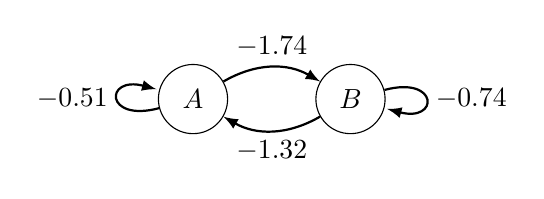
\begin{tikzpicture}[node distance=2cm,->,>=latex,auto,
  every edge/.append style={thick}]
  \node[state] (1) {$A$};
  \node[state] (2) [right of=1] {$B$};  
  \path (1) edge[loop left]  node{$-0.51$} (1)
            edge[bend left]  node{$-1.74$}   (2)
        (2) edge[loop right] node{$-0.74$}  (2)
            edge[bend left] node{$-1.32$}     (1);
\end{tikzpicture}
\end{center}
\begin{table}[h!]
\centering
\begin{tabular}{|l|l|l|}
\hline
\multicolumn{1}{|c|}{$x_t$} & \multicolumn{1}{c|}{$\log p(x_t|y_y=A)$} & $\log p(x_t|y_t=B)$ \\ \hline
X                           & -1                              & -1.74      \\ \hline
Y                           & -1.32                           & -1         \\ \hline
Z                           & -3.32                           & -2.32      \\ \hline
\end{tabular}
\end{table}

 We observed $x_1 = X$ and $x_2 = Y$. (Note that taking the maximum of log probabilities will give you the same result as taking the maximum of probabilities as log is a monotonically increasing function.)

\DIFdelbegin %DIFDELCMD < \clearpage
%DIFDELCMD < %%%
\DIFdelend \begin{questions}
    \DIFdelbegin %DIFDELCMD < \question[1] %%%
\DIFdelend \DIFaddbegin \question[2] \DIFaddend Compute $\log v_1(s_j=A)$ and $\log v_1(s_j=B)$. If your answers involves decimal numbers, please round your answer to \textbf{TWO} decimal places.

    $\log v_1(s_j=A):$ 
    \begin{tcolorbox}[fit,height=1cm, width=2cm, blank, borderline={1pt}{-2pt}]
            %solution 
    \end{tcolorbox}
    $\log v_1(s_j=B):$ 
    \begin{tcolorbox}[fit,height=1cm, width=2cm, blank, borderline={1pt}{-2pt}]
            %solution 
    \end{tcolorbox}

    
    \question[2] (\textbf{Select one}) Which of the following is the most likely sequence of hidden states? 
    \begin{checkboxes}
    \choice $y_1=A$, $y_2=A$
    \choice $y_1=A$, $y_2=B$
    \choice $y_1=B$, $y_2=A$
    \choice $y_1=B$, $y_2=B$
    \choice Don't have enough information.
    \end{checkboxes}

\end{questions}



\DIFdelbegin %DIFDELCMD < \clearpage
%DIFDELCMD < %%%
\DIFdelend \subsection{Warm-up Exercise: Forward-Backward Algorithm [4 pts]}\label{toy}
To help you prepare to implement the HMM forward-backward algorithm (see Section~\ref{forback} for a detailed explanation), we have provided a small example for you to work through by hand. This toy data set consists of a training set of three sequences with three unique words and two tags and a test set with a single sequence composed of the same unique words used in the training set. Before going through this example, please carefully read the algorithm description in Sections \ref{learn} and \ref{forback}. \textbf{Note:} pseudo count used in section 2 is also used here.

Training set:
\begin{verbatim}
you_B eat_A fish_B
you_B fish_B eat_A
eat_A fish_B
\end{verbatim}

Where the training word sequences are:
$$
x= 
\begin{bmatrix}
\text{you} & \text{eat} & \text{fish}\\
\text{you} & \text{fish} & \text{eat}\\
\text{eat} & \text{fish} &
\end{bmatrix}
$$

And the corresponding tags are:
$$
y= 
\begin{bmatrix}
\text{B} & \text{A} & \text{B}\\
\text{B} & \text{B} & \text{A}\\
\text{A} & \text{B} &
\end{bmatrix}
$$


Test set:
\begin{verbatim}
fish eat you
\end{verbatim}

or 
$$
x= 
\begin{bmatrix}
\text{fish} & \text{eat} & \text{you}\\
\end{bmatrix}
$$

The following four questions are meant to encourage you to work through the forward backward algorithm by hand using this test example. Feel free to use a calculator, being careful to carry enough significant figures through your computations to avoid rounding errors. For each question below, please report the requested value in the text box next to the question (these boxes are only visible in the template document). When a number is requested, only write the number in the box. When a word/tag is requested, only write that word or tag. \textbf{DO NOT} include explanations or derivation work in the text box. Points will be deducted if anything else is included in the box.

\DIFaddbegin \clearpage

\DIFaddend \begin{questions}
    \question[1] Compute $\alpha_2(A)$, the $\alpha$ value associated with the tag ``A'' for the second word in the test sequence. Please round your answer to \textbf{THREE} decimal places.

    \begin{tcolorbox}[fit,height=1cm, width=2cm, blank, borderline={1pt}{-2pt}]
            %solution 
        \end{tcolorbox}


    \question[1] Compute $\beta_2(B)$, the $\beta$ value associated with the tag ``B'' for the second word in the test sequence. Please round your answer to \textbf{THREE} decimal places.

    \begin{tcolorbox}[fit,height=1cm, width=2cm, blank, borderline={1pt}{-2pt}]
            %solution 
        \end{tcolorbox}

    \question[1] Predict the tag for the third word in the test sequence. 

    \begin{tcolorbox}[fit,height=1cm, width=2cm, blank, borderline={1pt}{-2pt}]
            %solution 
        \end{tcolorbox}

    \question[1] Compute the log-likelihood for the entire test sequence, ``\texttt{fish eat you}". Please round your answer to \textbf{THREE} decimal places.

    \begin{tcolorbox}[fit,height=1cm, width=2cm, blank, borderline={1pt}{-2pt}]
            %solution 
        \end{tcolorbox}

\end{questions}

\clearpage

\subsection{Empirical Questions [6 pts]}
\begin{notebox}
Return to these questions after implementing your \texttt{learnhmm.\{py|java|cpp|m\}} and 

\texttt{forwardbackward.\{py|java|cpp|m\}} functions.
\end{notebox}



Using the fulldata set \textbf{trainwords.txt} in the handout using your implementation of \texttt{learnhmm.\{py|java|cpp|m\}} to learn parameters for an hmm model using the first 10, 100, 1000, and 10000 sequences in the file.
Use these learned parameters perform prediction on the \textbf{trainwords.txt} and the \textbf{testwords.txt} files using your \texttt{forwardbackward.\{py|java|cpp|m\}}.
Construct a plot with number of sequences used for training on the x-axis (log-scale) and average log likelihood across all sequences from the \textbf{trainwords.txt} or the \textbf{testwords.txt} on the y-axis (see Section~\ref{forback} for details on computing the log data likelihood for a sequence). Each table entry is worth 0.5 points. 
Write the resulting log likelihood values in the table in the template.
Include your plot in the large box in the template (2 points).
To receive credit for your plot, you must submit a computer generated plot.
\textbf{DO NOT} hand draw your plot.

\begin{table}[h]
    \center
    \begin{tabular}{|m{2cm}|m{3cm}|m{3cm}|}
    \hline
    \#sequences & Train average log-likelihood & Test average log-likelihood \\ \hline
    10         &    &  \\ \hline
    100        &    &  \\ \hline
    1000       &    &  \\ \hline
    10000      &    &  \\ \hline
    \end{tabular}
    \end{table}

 \DIFdelbegin %DIFDELCMD < \begin{tcolorbox}[fit,height=12cm, width=17cm, blank, borderline={1pt}{-2pt}]
%DIFDELCMD <     %%%
\DIFdelend \DIFaddbegin \begin{tcolorbox}[fit,height=13cm, width=17cm, blank, borderline={1pt}{-2pt}]
    \DIFaddend %solution 
 \end{tcolorbox}

\newpage
\subsection{Collaboration Policy}
After you have completed all other components of this assignment, report your answers to the collaboration policy questions detailed in the Academic Integrity Policies found \href{http://www.cs.cmu.edu/~mgormley/courses/10601bd-f18/about.html#7-academic-integrity-policies}{here}.
    \begin{enumerate}
        \item Did you receive any help whatsoever from anyone in solving this assignment? Is so, include full details.
        \item Did you give any help whatsoever to anyone in solving this assignment? Is so, include full details.
        \item Did you find or come across code that implements any part of this assignment ? If so, include full details.
    \end{enumerate}

\begin{tcolorbox}[fit,height=10cm, width=17cm, blank, borderline={1pt}{-2pt}]
    %solution 
    \end{tcolorbox}

\clearpage\section{Programming [80 pts]}
\label{programming}

\subsection{The Tasks and Data Sets}\label{dataset}
The handout file for this assignments contains several files that you will use in the homework. The contents and formatting of each of these files is explained below\DIFdelbegin \DIFdel{(these files are organized in two folders for the full and toy dataset, with corresponding prefixes)}\DIFdelend .
\begin{enumerate}

\item \textbf{trainwords.txt} This file contains labeled text data that you will use in training your model in the \textbf{Learning} problem. Specifically the text contains one sentence per line that has already been preprocessed, cleaned and tokenized. You should treat every line as a separate sequence and assume that it has the following format:

    \texttt{<Word0>\_<Tag0> <Word1>\_<Tag1> ... <WordN>\_<TagN>}

where every \texttt{<WordK>\_<TagK>} unit token is separated by white space.

\item \textbf{testwords.txt}: This file contains labeled data that you will use to evaluate your model in the \textbf{Experiments} section. This file contains the gold standard labels.  This file has the same format as \textbf{trainwords.txt}.

\item \textbf{index\_to\_word.txt} and \textbf{index\_to\_tag.txt}: These files contain a list of all words or tags that appear in the data set. In your functions, you will convert the string representation of words or tags to indices corresponding to the location of the word or tag in these files. For example, if Austria is on line 729 of \textbf{index\_to\_word.txt}, then all appearances of Austria in the data sets should be converted to the index 729. This index will also correspond to locations in the parameter matrices. For example, the word Austria corresponds to the parameters in column 729 of the matrix stored in \textbf{hmmemit.txt}. This will be useful for your forward-backward algorithm implementation (see Section~\ref{forback}).

\item \textbf{toytrain.txt}, \textbf{toytest.txt}, \textbf{toy\_index\_to\_word.txt}, and \textbf{toy\_index\_to\_tag.txt}: These files are analogous to \textbf{trainwords.txt}, \textbf{testwords.txt}, \textbf{index\_to\_word.txt}, and \textbf{index\_to\_tag.txt} and are used to compare your implementation to your hand calculations in Section~\ref{toy}.

\item \textbf{predicttest.txt} The \textbf{predicttest.txt} file contains labeled data that you will use to debug your implementation. The labels in this file are not gold standard but are generated by running our decoder using the features from \textbf{trainwords.txt}. This file has the same format as \textbf{trainwords.txt}.

\item \textbf{metrics.txt} The \textbf{metrics.txt} file contains the metrics you will compute for the dataset. For this assignment, you need to compute the average log likelihood and your prediction accuracy on the test data. Note that in Named Entity Recognition, F-1 score is a more common metric to evaluate the model performance, here you only need to report your accuracy for tag prediction of each word. 

Sample metrics file for the toy dataset


\item \textbf{hmmtrans.txt, hmmemit.txt and hmmprior.txt}: These files contain pre-trained model parameters of an HMM that you will use in testing your implementation of the \textbf{Learning} and \textbf{Evaluation and Decoding} problems. The format of the first two files are analogous and is as follows. Every line in these files consists of a conditional probability distribution. In the case of transition probabilities, this distribution corresponds to the probability of transitioning into another state, given a current state. Similarly, in the case of emission probabilities, this distribution corresponds to the probability of emitting a particular symbol, given a current state. For example, every line in \textbf{hmmtrans.txt} has the following format:

    \textbf{hmmtrans.txt}:\\
    \texttt{<ProbS1S1> ... <ProbS1SN>}\\
     \texttt{<ProbS2S1> ... <ProbS2SN>}...\\   

and every line in \textbf{hmmemit.txt} has the following format:

    \textbf{hmmemit.txt}:\\
    \texttt{<ProbS1Word1> ... <ProbS1WordN>}\\
     \texttt{<ProbS2Word1> ... <ProbS2WordN>}...\\

In both cases, elements in the same row are separated by white space. Each row corresponds to a line of text (using \texttt{\char`\\ n} to create new lines).

    
The format of \textbf{hmmprior.txt} is similarly defined except that it only contains a single probability distribution over starting states. Therefore each row only has a single element. Therefore \textbf{hmmprior.txt} has the following format:

    \textbf{hmmprior.txt}:\\
    \texttt{<ProbS1>}\\
     \texttt{<ProbS2>}...\\

\end{enumerate}

Note that the data provided to you is to help in developing your implementation of the HMM algorithms. Your code will be tested on Autolab using different data with different HMM parameters, likely coming from a different domain although the format will be identical.

\subsection{Learning}\label{learn}
Your first task is to implement an algorithm to learn the hidden Markov model parameters needed to apply the forward backward algorithm (See Section \ref{forback}). There are three sets of parameters that you will need to estimate: the initialization probabilities {\boldmath$\pi$}, the transition probabilities $\mathbf A$, and the emission probabilities $\mathbf B$. For this assignment, we model each of these probabilities using a multinomial distribution with parameters $ \pi_j=P(y_1=j)$, $ a_{jk} = P(y_{t}=k\vert y_{t-1}=j)$, and $ b_{jk} = P(x_t=k\vert y_{t}=j)$. These can be estimated using maximum likelihood, which results in the following parameter estimators:

\begin{enumerate}
    \item $P(y_1 = j) = \pi_j = \frac{N_\pi^j+1}{\sum_{p=1}^{J}(N_\pi^p+1)}$, where $N_\pi^j$ equals the number of times state $s_j$ is associated with the first word of a sentence in the training data set.
    \item $P(y_{t} = k\vert y_{t-1}=j) = a_{jk}= \frac{N_A^{jk}+1}{\sum_{p=1}^J (N_A^{jp}+1)}$, where $N_A^{jk}$ is the number of times state $s_j$ is followed by state $s_k$ in the training data set.  
    \item $P(x_{t} = k\vert y_{t}=j) = b_{jk}= \frac{N_B^{jk}+1}{\sum_{p=1}^M (N_B^{jp}+1)}$, where $N_B^{jk}$ is the number of times that the state $s_j$ is associated with the word $k$ in the training data set.
\end{enumerate}

Note that for each count, a ``+1'' is added to make a \textbf{pseudocount}. This is slightly different from pure maximum likelihood estimation, but it is useful in improving performance when evaluating unseen cases during evaluation of your test set.

You should implement a function that reads in the training data set (\textbf{trainwords.txt}), and then estimates $\pi$, $A$, and $B$ using the above maximum likelihood solutions. 

Your outputs should be in the same format as \textbf{hmmprior.txt}, \textbf{hmmtrans.txt}, and \textbf{hmmemit.txt} (including the same number of decimal places to ensure there are no rounding errors during prediction). The autograder will use the following commands to call your function:

\begin{tabbing}
For Python: \=\texttt{\$ \textbf{python} learnhmm.\textbf{py} [args\dots]}\\
For Java: \>\texttt{\$ \textbf{javac} -cp "./lib/ejml-v0.33-libs/*:./" learnhmm.\textbf{java};\DIFaddbegin }\DIFaddend \\
          \>  \DIFdelbegin \texttt{\textbf{\DIFdel{java}} %DIFAUXCMD
\DIFdel{-cp "./lib/ejml-v0.33-libs/*:./" learnhmm }%DIFDELCMD < [%%%
\DIFdel{args}%DIFDELCMD < \dots]%%%
}%DIFAUXCMD
%DIFDELCMD < \MBLOCKRIGHTBRACE%%%
\DIFdelend \DIFaddbegin \texttt{\DIFadd{\$ }\textbf{\DIFadd{java}} \DIFadd{-cp "./lib/ejml-v0.33-libs/*:./" learnhmm }[\DIFadd{args}\dots]}\DIFaddend \\
For C++: \>\texttt{\$ \textbf{g++} -g -std=c++11 -I./lib learnhmm.\textbf{cpp}; ./a.out [args\dots]}\\
For Octave: \>\texttt{\$ \textbf{octave} -qH learnhmm.\textbf{m} [args\dots]}
\end{tabbing}

Where above \texttt{[args\dots]} is a placeholder for six command-line arguments:\texttt{<train\_input>} \texttt{<index\_to\_word>} \texttt{<index\_to\_tag>} \texttt{<hmmprior>} \texttt{<hmmemit>} \texttt{<hmmtrans>}. These arguments are described in detail below:
\begin{enumerate}
    \item \texttt{<train\_input>}: path to the training input \texttt{.txt} file (see Section~\ref{dataset})
    \item \texttt{<index\_to\_word>}: path to the \texttt{.txt} that specifies the dictionary mapping from words to indices. The tags are ordered by index, with the first word having index of 1, the second word having index of 2, etc.
    \item \texttt{<index\_to\_tag>}: path to the \texttt{.txt} that specifies the dictionary mapping from tags to indices. The tags are ordered by index, with the first tag having index of 1, the second tag having index of 2, etc.
    \item \texttt{<hmmprior>}: path to output \texttt{.txt} file to which the estimated prior (\boldmath${\pi}$) will be written. The file output to this path should be in the same format as the handout \texttt{hmmprior.txt} (see Section~\ref{dataset}).
    \item \texttt{<hmmemit>}: path to output \texttt{.txt} file to which the emission probabilities ($\mathbf B$) will be written. The file output to this path should be in the same format as the handout \texttt{hmmemit.txt} (see Section~\ref{dataset})
    \item \texttt{<hmmtrans>}: path to output \texttt{.txt} file to which the transition probabilities ($\mathbf A$) will be written. The file output to this path should be in the same format as the handout \texttt{hmmtrans.txt} (see Section~\ref{dataset})..
\end{enumerate}


\subsection{Evaluation and Decoding}
\label{forback}

\subsubsection{Forward Backward Algorithm and Minimal Bayes Risk Decoding}

Your next task is to implement the forward-backward algorithm. Suppose we have a set of sequence consisting of $T$ words, $x_1,...,x_T$. Each word is associated with a label $y_t\in\{1,...,J\}$. In the forward-backward algorithm we seek to approximate $P(y_t | x_1,...,x_T)$ up to a multiplication constant. This is done by first breaking $P(y_t | x_1,...,x_T)$ into a ``forward'' component and a ``backward'' component as follows:
\begin{align*}
   P(y_t =s_j | x_1,...,x_T) &\propto P(y_t=s_j,x_{t+1},...,x_T|x_1,...,x_{t})\\
   &\propto P(y_t=s_j|x_1,...,x_{t})P(x_{t+1},...,x_T|y_t=s_j, x_1,...,x_{t})\\
    &\propto P(y_t=s_j|x_1,...,x_{t})P(x_{t+1},...,x_T|y_t=s_j)\\ 
     &\propto P(y_t=s_j, x_1,...,x_{t})P(x_{t+1},...,x_T|y_t=s_j) 
\end{align*}

where $P(y_t=s_j|x_1,...,x_{t})$ is computed by passing forward recursively through the model and $P(x_{t+1},...,x_T|y_t=j)$ is computed by passing recursively backwards through the model.

\newpage
\textbf{Forward Algorithm}

Define $\alpha_t(j) = P(y_t = j, x_{1:t})$. We can rearrange our definition of $\alpha_t(j)$ as follows:
\begin{align}
    \label{eqn:alpha}
    \alpha_t(j)
    =&P(y_t=s_j, x_{1:t}) \nonumber\\
    =& \sum_{k} P(y_t=s_j, y_{t-1}=s_k, x_{1:t}) \nonumber\\
    =& \sum_{k} P(y_{t-1}=s_k, x_{1:t} \vert y_t = s_j) P(y_t = s_j) \nonumber\\
    =& \sum_{k} P(x_t \vert y_t = s_j) P(y_{t-1}=s_k, x_{1:t-1} \vert y_t = s_j) P(y_t = s_j) \nonumber\\
    =& P(x_t \vert y_t = s_j) \sum_{k} P(y_t = s_j, y_{t-1}=s_k, x_{1:t-1}) \nonumber\\
    =& P(x_t \vert y_t = s_j) \sum_{k} P(y_t = s_j, x_{1:t-1} \vert y_{t-1}=s_k) P(y_{t-1}=s_k) \nonumber\\
    =& P(x_t \vert y_t = s_j) \sum_{k} P(y_t = s_j \vert y_{t-1}=s_k) P(x_{1:t-1} \vert y_{t-1}=s_k) P(y_{t-1}=s_k) \nonumber\\
    =& P(x_t \vert y_t = s_j) \sum_{k} P(y_t = s_j \vert y_{t-1}=s_k) P(y_{t-1}=s_k, x_{1:t-1}) \nonumber\\
    =& b_{jx_t} \sum_{k} a_{kj} \alpha_{t-1}(k)
\end{align}


Using this definition, the $\alpha$'s can be computed using the following recursive procedure:
\begin{enumerate}
    \item $\alpha_1(j)=\pi_jb_{jx_1}$. 
    \item For $t > 1$, $\alpha_{t}(j)=b_{jx_{t}}\sum_{k=1}^{J}\alpha_{t-1}(k)a_{kj}$ 
\end{enumerate}


\textbf{Backward Algorithm}
Define $\beta_t(j) = P(x_{t+1},...,x_T|y_t=s_j)$. We can rearrange our definition of $\beta_t(j)$ as follows:

\begin{align}
    \label{eqn:beta}
    \beta_t(j) &= P(x_{t+1},...,x_T|y_t=s_j)\nonumber\\
    &= \sum_{k=1}^JP(y_{t+1}=s_k,x_{t+1},...,x_T|y_t=s_j)\nonumber\\
    &= \sum_{k=1}^JP(x_{t+1},...,x_T|y_t=s_j,y_{t+1}=s_k)P(y_{t+1}=s_k|y_t=s_j)\nonumber\\
    &= \sum_{k=1}^JP(x_{t+1}|y_{t+1}=s_k)P(x_{t+2},...,x_T|y_{t+1}=s_k)P(y_{t+1}=s_k|y_t=s_j)\nonumber\\
    &= \sum_{k=1}^J b_{kx_{t+1}}\beta_{t+1}(k)a_{jk}
\end{align}


Just like the $\alpha$'s, the $\beta$'s can also be computed using the following backward recursive procedure:

\begin{enumerate}
    \item $\beta_T(j) = 1$ (All states could be ending states)
    \item  For $1\leq t <T$, $\beta_t(j) = \sum_{k=1}^{J}b_{kx_{t+1}}\beta_{t+1}(k)a_{jk}$ (Generate $x_{t+1}$ from any state)
\end{enumerate}


\textbf{Forward-Backward Algorithm}
As stated above, the goal of the Forward-Backward algorithm is to compute $P(y_t =s_j | x_1,...,x_T)$. This can be done using the following equation:

$$P(y_t =s_j | x_1,...,x_T) \propto P(y_t=s_j, x_1,...,x_{t})P(x_{t+1},...,x_T|y_t=s_j) $$

After running your forward and backward passes through the sequence, you are now ready to estimate the conditional probabilities as:

$$P(y_t | x_1,...,x_T) \propto \alpha_t\circ\beta_t$$
where $\circ$ is the element-wise product.

\textbf{Minimum Bayes Risk Prediction}
We will assign tags using the minimum Bayes risk predictor, defined for this problem as follows:

$$\hat{y}_t = \argmax_{j\in \{1,...,J\}} P(y_t = s_j\vert x_1,...,x_T)$$

To resolve ties, select the tag that appears earlier in the \texttt{<index\_to\_tag>} input file.

\textbf{Computing the Log Likelihood of a Sequence}
When we compute the log likelihood of a sequence, we are interested in the computing the quantity $P(x_1,...,x_T)$. We can rewrite this in terms of values we have already computed in the forward-backward algorithm as follows:

\begin{align*}
    \log P(x_1,...,x_T) &= \log\big(\sum_j P(x_1,...,x_T,y_T=s_j)\big)\\
    &= \log\big(\sum_j \alpha_T(j)\big)
\end{align*}

\subsubsection{Implementation Details}

You should now implement your forward-backward algorithm as a program, \texttt{forwardbackward.\{py|java|cpp|m\}}. The program will read in test data and the parameter files produced by \texttt{learnhmm.\{py|java|cpp|m\}}. The autograder will use the following commands to call your function:

\begin{tabbing}
For Python: \=\texttt{\$ \textbf{python} forwardbackward.\textbf{py} [args\dots]}\\
For Java: \>\texttt{\$ \textbf{javac} -cp "./lib/ejml-v0.33-libs/*:./" forwardbackward.\textbf{java}\DIFaddbegin }\DIFaddend ;\\ 
          \>\texttt{\textbf{java} -cp "./lib/ejml-v0.33-libs/*:./" forwardbackward [args\dots]}\DIFdelbegin %DIFDELCMD < \MBLOCKRIGHTBRACE%%%
\DIFdelend \\
For C++: \>\texttt{\$ \textbf{g++} -g -std=c++11 -I./lib forwardbackward.\textbf{cpp}; ./a.out [args\dots]}\\
For Octave: \>\texttt{\$ \textbf{octave} -qH \DIFdelbegin \DIFdel{forwardbackward}\DIFdelend \DIFaddbegin \DIFadd{forwardBackward}\DIFaddend .\textbf{m} [args\dots]}
\end{tabbing}

Where above \texttt{[args\dots]} is a placeholder for seven command-line arguments:\texttt{<test\_input>} \texttt{<index\_to\_word>} \texttt{<index\_to\_tag>} \texttt{<hmmprior>} \texttt{<hmmemit>} \texttt{<hmmtrans>} \texttt{<predicted\_file>} \texttt{<metric\_file>}. These arguments are described in detail below:
\begin{enumerate}
    \item \texttt{<test\_input>}: path to the test input \texttt{.txt} file that will be evaluated by your forward backward algorithm (see Section~\ref{dataset})
    \item \texttt{<index\_to\_word>}: path to the \texttt{.txt} that specifies the dictionary mapping from words to indices. The tags are ordered by index, with the first word having index of 1, the second word having index of 2, etc. This is the same file as was described for \texttt{learnhmm.\{py|java|cpp|m\}}.
    \item \texttt{<index\_to\_tag>}: path to the \texttt{.txt} that specifies the dictionary mapping from tags to indices. The tags are ordered by index, with the first tag having index of 1, the second tag having index of 2, etc. This is the same file as was described for \texttt{learnhmm.\{py|java|cpp|m\}}.
    \item \texttt{<hmmprior>}: path to input \texttt{.txt} file which contains the estimated prior (\boldmath${\pi}$).
    \item \texttt{<hmmemit>}: path to input \texttt{.txt} file which contains the emission probabilities ($\mathbf B$).
    \item \texttt{<hmmtrans>}: path to input \texttt{.txt} file which contains transition probabilities ($\mathbf A$).
    \item \texttt{<predicted\_file>}: path to the output \texttt{.txt} file to which the predicted tags will be written. The file should be in the same format as the \texttt{<test\_input>} file. 
    \item \texttt{<metric\_file>}: path to the output \texttt{.txt} file to which the metrics will be written. 
\end{enumerate}


Example command for python users:
\begin{lstlisting}
$ python forwardbackward.py toydata/toytrain.txt \
toydata/toy_index_to_word.txt toydata/toy_index_to_tag.txt hmmprior.txt \
hmmemit.txt hmmtrans.txt predicted.txt metrics.txt
\end{lstlisting}

After running the command above, the \texttt{<predicted\_file>} output should be:

\begin{lstlisting}
you_B eat_A fish_B
you_B fish_B eat_A
eat_A fish_B
\end{lstlisting}

And the \texttt{<metric\_file>} output should be:

\begin{lstlisting}
Average Log-Likelihood: -2.776793
Accuracy: 1.0
\end{lstlisting}

Take care that your output has the exact same format as shown above. There should be a single space after the colon preceding the metric value (e.g. a space after \lstinline{Average Log-Likelihood:}). Each line should be terminated by a Unix line ending \lstinline{\n}.



\subsubsection{Log-Space Arithmetic for Avoiding Underflow}
\label{sec:underflow}

Handling underflow properly is a critical step in implementing an HMM. And the most generalized way of handling numerical underflow due to products of small positive numbers (like probabilities) is to calculate everything in \textbf{log-space}, i.e., represent every quantity by their logarithm, 

For this homework, using log-space trick starts with transforming Eq.(\ref{eqn:alpha}) and Eq.(\ref{eqn:beta}) into logarithmic form (how to do that is straightforward and left as an exercise). Please use $e$ as the base for logarithm calculation (natural log).

After transforming the equations into log form, you may discover calculation of the following type:

$$ \log \sum_i \exp{(v_i)}$$

This may be programmed as is, but $\exp{(v_i)}$ may cause underflow when $v_i$ is large and negative. One way to avoid this is to use the \href{https://www.xarg.org/2016/06/the-log-sum-exp-trick-in-machine-learning/}{log-sum-exp trick}. We provide the pseudo code for this trick in Algorithm \ref{alg:logsumexp}:

\begin{algorithm}[H] 
 \DIFdelbegin %DIFDELCMD < \caption{%
{%DIFAUXCMD
\DIFdel{Log-Sum-Exp Trick}}
  %DIFAUXCMD
\DIFdelend \label{alg:logsumexp}
 \DIFdelbegin %DIFDELCMD < \begin{algorithmic}[1]
%DIFDELCMD <     \Procedure{logsumexp}{$v_1, v_2, \cdots, v_n$}
%DIFDELCMD <         \State %%%
\DIFdelend \DIFaddbegin \SetKwInOut{Input}{Input}
 \SetKwInOut{Output}{Return}
 \Input{$v_1, v_2, \cdots, v_n$}
 \DIFaddend $m = \max(v_i)$ \DIFdelbegin \DIFdel{,  }\DIFdelend \DIFaddbegin \DIFadd{; \;
 }\DIFaddend $i=\{1, 2,\cdots, n\}$ \DIFdelbegin %DIFDELCMD < \State \textbf{%%%
\DIFdel{return}%DIFDELCMD < \MBLOCKRIGHTBRACE %%%
\DIFdelend \DIFaddbegin \DIFadd{; \;
 }\textbf{\DIFadd{Return: }}{\DIFaddend $m + \log(\sum_i\exp(v_i-m))$\DIFdelbegin %DIFDELCMD < \EndProcedure
%DIFDELCMD <   \end{algorithmic}
%DIFDELCMD < %%%
\DIFdelend \DIFaddbegin } 
 \caption{\DIFadd{Log-Sum-Exp Trick}}
\DIFaddend \end{algorithm}
\DIFaddbegin 


\DIFaddend \subsection{Gradescope Submission}

You should submit your \texttt{learnhmm.\{py|m|java|cpp\}} and %\newline 
\texttt{forwardbackward.\{py|m|java|cpp\}} to Gradescope.
Note: please do not use other file names. This will cause problems for the autograder to correctly detect and run your code.

Some additional tips: 
Make sure to read the autograder output carefully. The autograder for Gradescope prints out some additional 
information about the tests that it ran\DIFaddbegin \DIFadd{. For this programming assignment we've specially designed some buggy implementations that you might do, and try our best to detect those and give you some more useful feedback in Gradescope's autograder}\DIFaddend . Make wise use of autograder's output for debugging your code. 

Note: For this assignment, you may make up to 10 submissions to Gradescope before the deadline, but only your last submission will be graded.

    
%%%%%%%%%%%%%%%%%%%%%%%%%%%%%%%%%%%%%%%%%%%%%%%%%%%%%%%%%%%%%%%%%%%%%%%%%%%%%%%%%%%




\end{document}